\documentclass{article}
\usepackage{luatextra}
\usepackage{polyglossia}
\usepackage{ulem}
\usepackage{framed}
\usepackage{color}
\usepackage{geometry}
\usepackage{amsmath}
\usepackage{unicode-math}
\usepackage[hidelinks]{hyperref}
\usepackage{latexsym}
\usepackage{pdflscape}
\usepackage{pdfpages}
\usepackage{enumitem}
\usepackage{titlesec}
\usepackage{lastpage}
\usepackage{fancyhdr}

\usepackage{ifluatex}
\ifluatex
  \usepackage{pdftexcmds}
  \makeatletter
  \let\pdfstrcmp\pdf@strcmp
  \let\pdffilemoddate\pdf@filemoddate
  \makeatother
\fi
\usepackage{svg}


\setmainlanguage{french}
\selectlanguage{french}
\setdefaultlanguage{french}
%%\setmainfont{Latin Modern Roman}
\setmainfont{Roboto}

\geometry{margin={1in,1in}}


\setlist{nosep} %% No space between lists' items

\pagestyle{fancy}
\fancyhead[R]{}

%% <current page>/<total pages> footer
\cfoot{\thepage/\pageref{LastPage}}

\newcommand\image[2]{
\directlua{
local image = img.scan({filename = "#1"})

image.height = image.height * #2
image.width  = image.width  * #2

node.write(img.node(image))
}
}


%%%%%%%%%%%%%%%%%%%%%%%%%%%%%%%%%%%%%%%%%%
%% \subsubsubsection command definition %%
%%%%%%%%%%%%%%%%%%%%%%%%%%%%%%%%%%%%%%%%%%


\titleclass{\subsubsubsection}{straight}[\subsection]

\newcounter{subsubsubsection}[subsubsection]
\renewcommand\thesubsubsubsection{\thesubsubsection.\arabic{subsubsubsection}}
\renewcommand\theparagraph{\thesubsubsubsection.\arabic{paragraph}} % optional; useful if paragraphs are to be numbered

\titleformat{\subsubsubsection}
  {\normalfont\normalsize\bfseries}{\thesubsubsubsection}{1em}{}
\titlespacing*{\subsubsubsection}
{0pt}{3.25ex plus 1ex minus .2ex}{1.5ex plus .2ex}

\makeatletter
\renewcommand\paragraph{\@startsection{paragraph}{5}{\z@}%
  {3.25ex \@plus1ex \@minus.2ex}%
  {-1em}%
  {\normalfont\normalsize\bfseries}}
\renewcommand\subparagraph{\@startsection{subparagraph}{6}{\parindent}%
  {3.25ex \@plus1ex \@minus .2ex}%
  {-1em}%
  {\normalfont\normalsize\bfseries}}
\def\toclevel@subsubsubsection{4}
\def\toclevel@paragraph{5}
\def\toclevel@paragraph{6}
\def\l@subsubsubsection{\@dottedtocline{4}{7em}{4em}}
\def\l@paragraph{\@dottedtocline{5}{10em}{5em}}
\def\l@subparagraph{\@dottedtocline{6}{14em}{6em}}
\makeatother

\setcounter{secnumdepth}{4}
\setcounter{tocdepth}{4}

%%%%%%%%%%%%%%%%%%%%%%%%%%%%%%%%%%%%%%%%%%
%% end \subsubsubsection definition     %%
%%%%%%%%%%%%%%%%%%%%%%%%%%%%%%%%%%%%%%%%%%

\title{COO — Équipe 6}
\author{Cancela Joël\\Bounouas Nassim\\Mortara Johann\\Novac Pierre-Emmanuel}


\begin{document}
% a

\maketitle
\tableofcontents


\section{Choix de conception}

\section{Diagramme de cas d'utilisation}

\vspace{-5em}
\hspace*{-8em}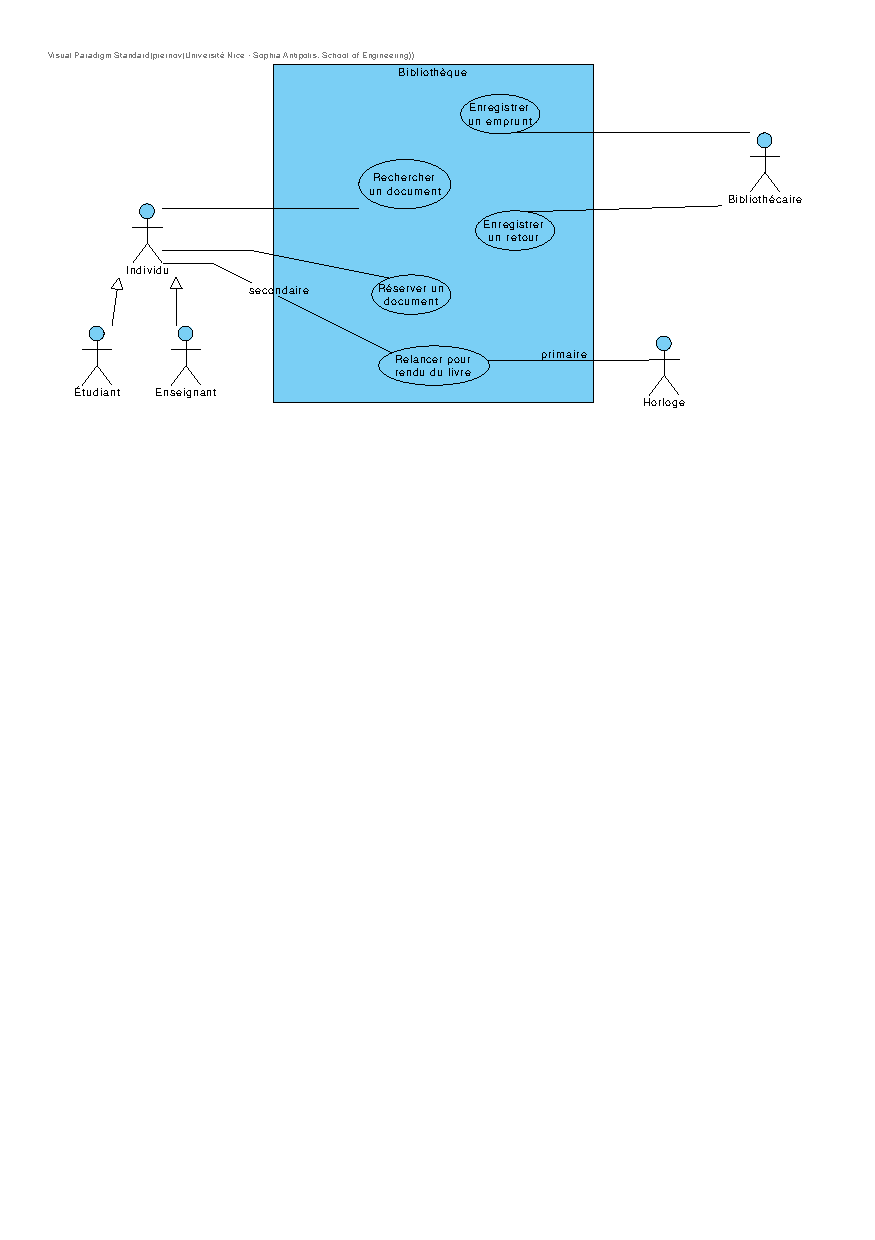
\includegraphics[scale=1.5]{use_case}
\vspace*{-4em}

\section{Cas d'utilisation: Emprunter un livre}

\noindent\textbf{Nom:} Emprunter un livre \\
\textbf{Description:} La bibliothécaire enregistre l'emprunt d'un livre.\\
\textbf{Précondition:} La bibliothécaire dispose du numéro du livre et du numéro de l'individu.\\
\textbf{Postcondition:} L'emprunt est validé.\\
\textbf{Cas d'erreur:} Le livre n’existe pas, le livre est déjà emprunté, l’individu n’existe pas, l’individu est suspendu ou l’individu a déjà emprunté 3 livres.\\
\textbf{État du système en cas d'erreur:} L’emprunt n'est pas validé.\\
\textbf{Acteurs:} La bibliothécaire \\
\textbf{Déclenchement:} La bibliothécaire reçoit une demande d'emprunt d'un livre de la part d'un individu.\\
\textbf{Scénario primaire:}
\begin{enumerate}
	\item La bibliothécaire entre le numéro du document et le numéro de l'individu dans l'interface de la Bibliothèque.
	\item La Bibliothèque recherche l'individu dans l'Annuaire.
	\item La Bibliothèque recherche le livre dans le Fonds de bibliothèque.
	\item Le livre est disponible, l'étudiant n'est pas suspendu et a moins de 3 emprunts.
	\item La Bibliothèque enregistre l'emprunt.
\end{enumerate}

\noindent\textbf{Scénario alternatif:}
\begin{itemize}
	\item[2'.] L’étudiant n’existe pas, fin du cas d’utilisation.
	\item[3'.] Le livre n’existe pas, fin du cas d’utilisation.
	\item[4'.] Le livre est déjà emprunté, l’individu est suspendu ou l’individu a déjà emprunté 3 livres, fin du cas d’utilisation.
\end{itemize}


\section{Diagramme de classes}

\vspace{-5em}
\hspace*{-9em}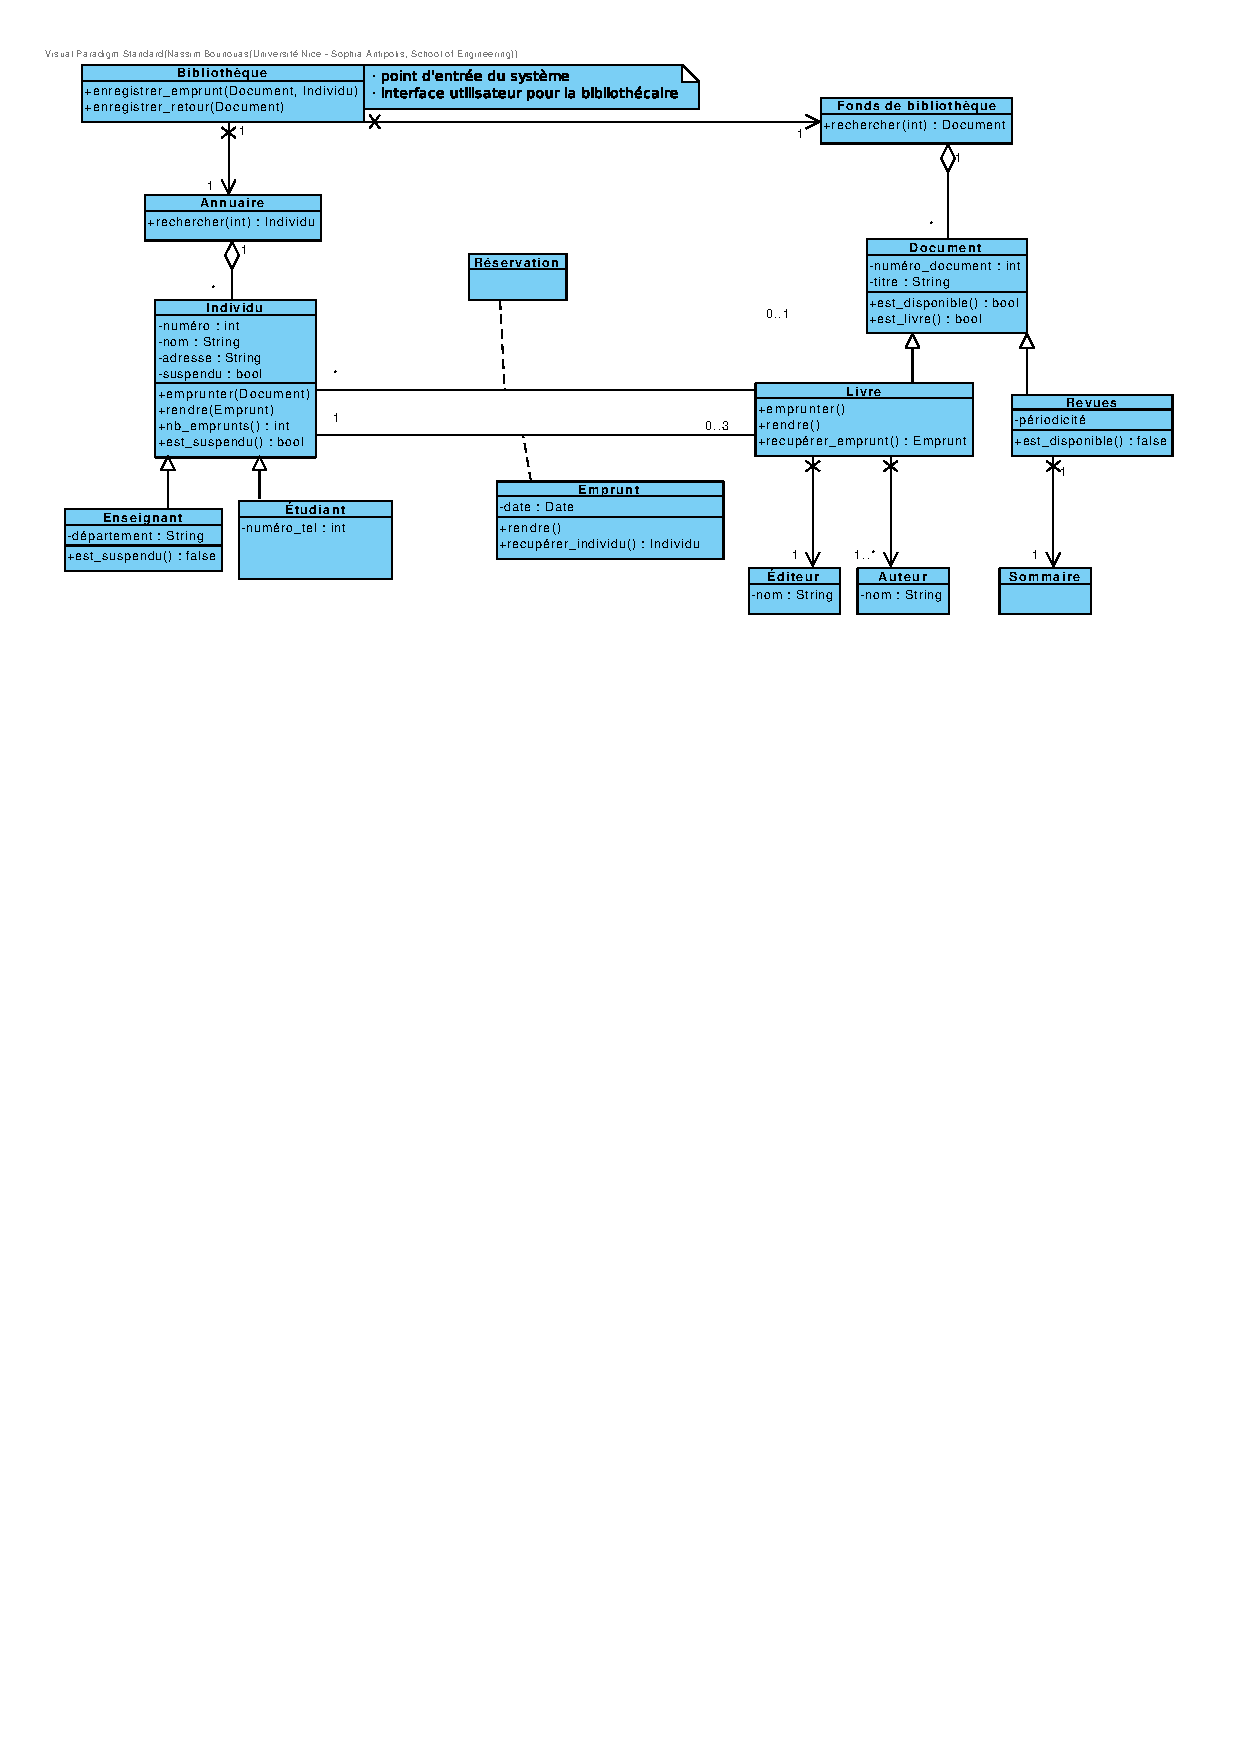
\includegraphics[scale=1.5]{class}
\vspace*{-4em}

\section{Diagrammes de séquence}

\subsection{Enregistrer un emprunt}
\vspace{-5em}
\hspace*{-10em}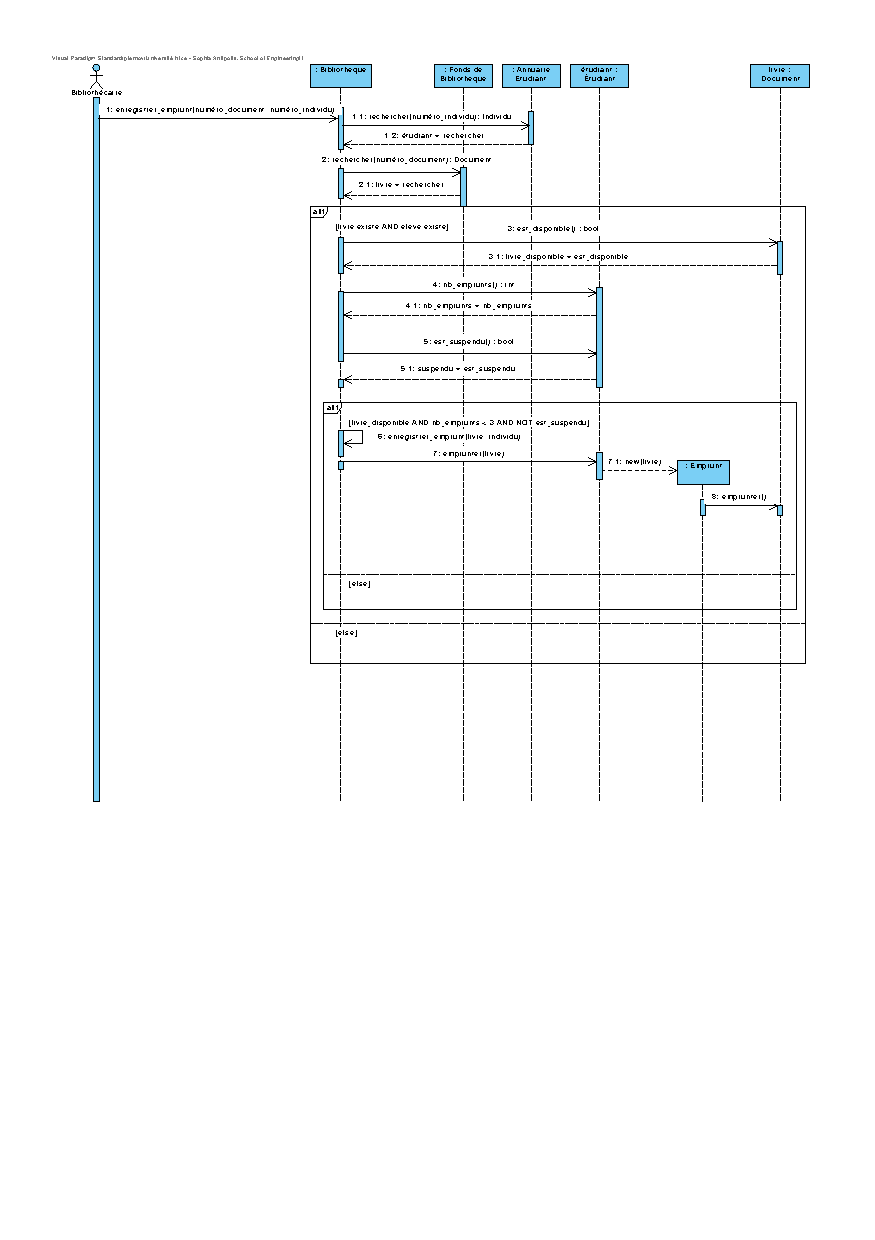
\includegraphics[scale=1.56]{sequence_enregistrer_un_emprunt}
\vspace*{-4em}

\subsection{Enregistrer un retour}
\vspace{-4em}
\hspace*{-9em}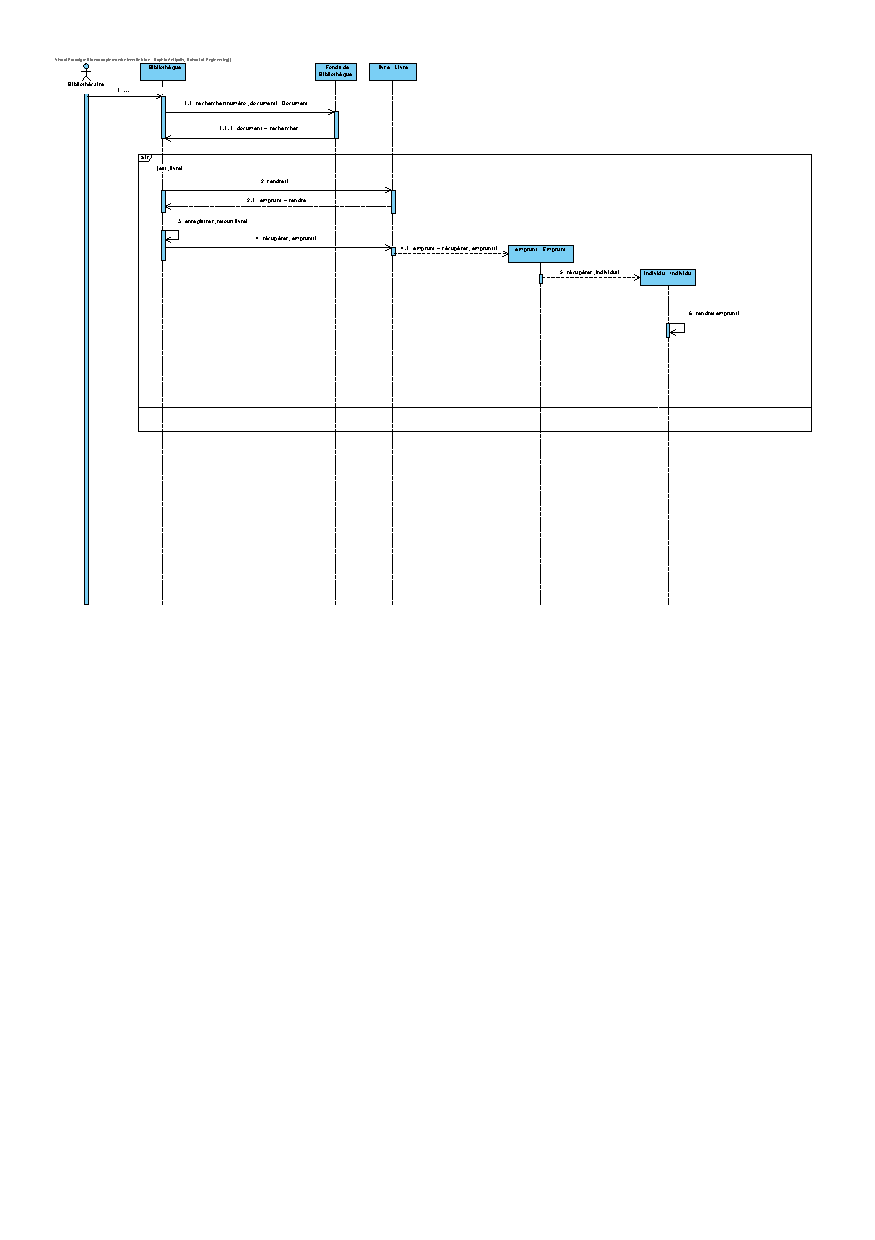
\includegraphics[scale=1.5]{sequence_enregistrer_un_retour}
\vspace*{-4em}

\subsection{Rechercher un document}
\vspace{-4em}
\hspace*{-9em}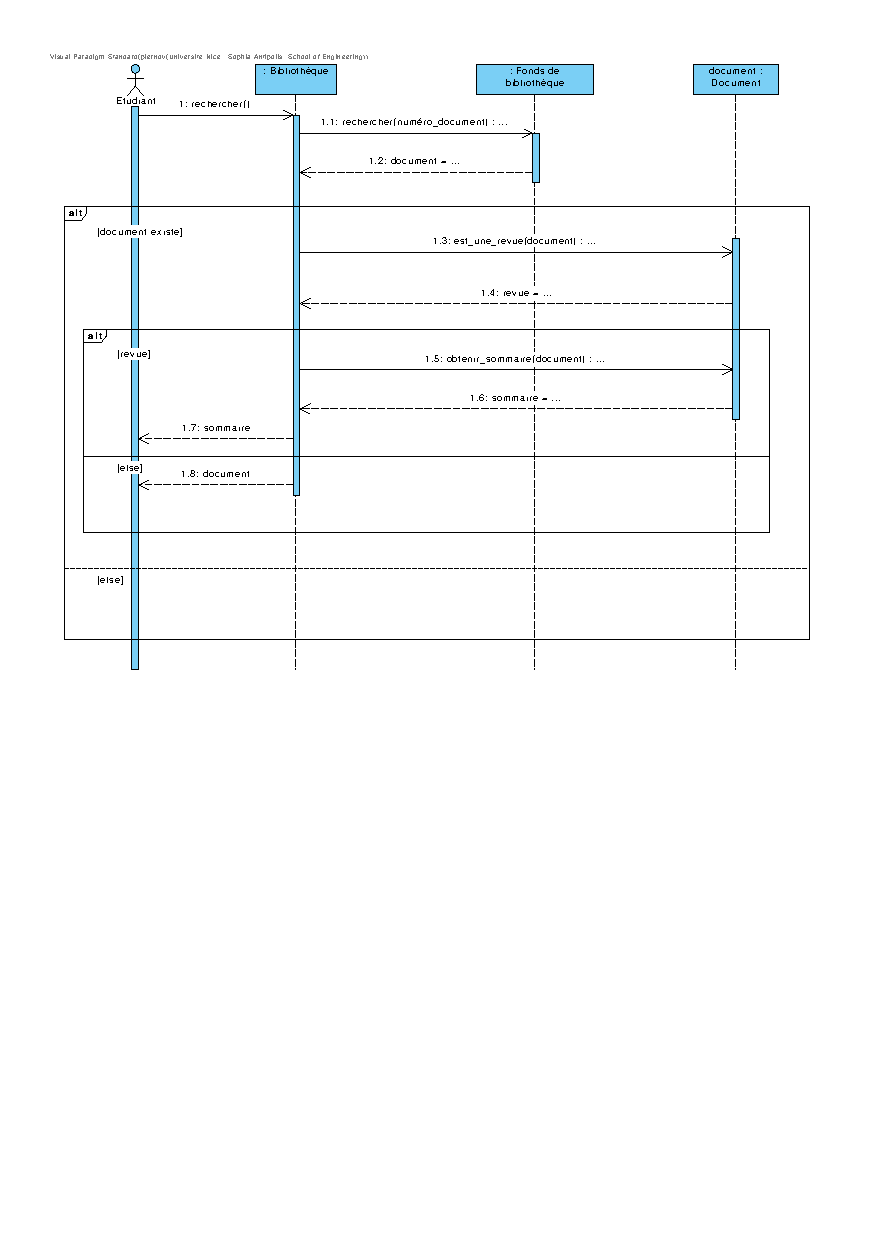
\includegraphics[scale=1.5]{sequence_rechercher_un_document}
\vspace*{-4em}

\subsection{Réserver un livre}
\vspace{-5em}
\hspace*{-10em}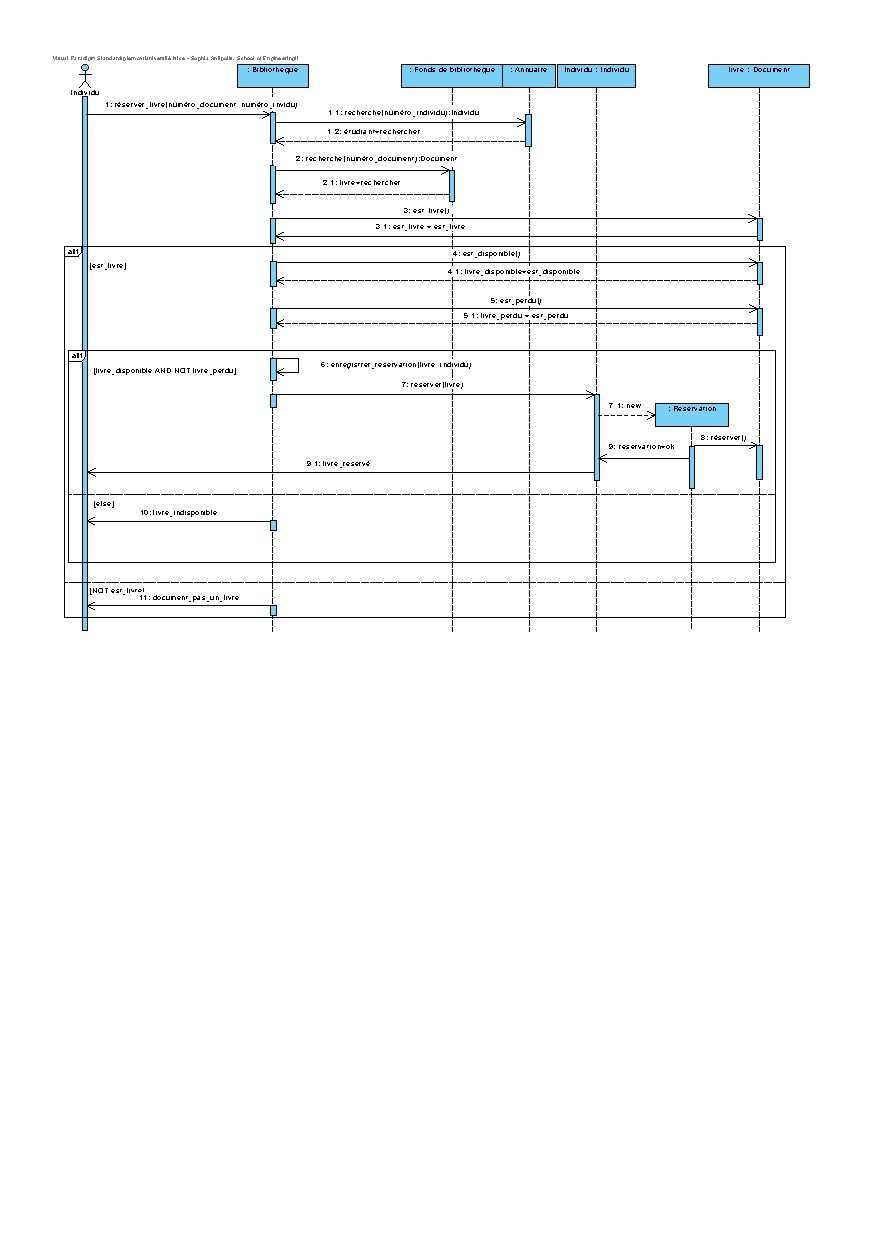
\includegraphics[scale=1.56]{sequence_reserver_un_livre}
\vspace*{-4em}

\subsection{Relancer pour rendu du livre}
\vspace{-4em}
\hspace*{-9em}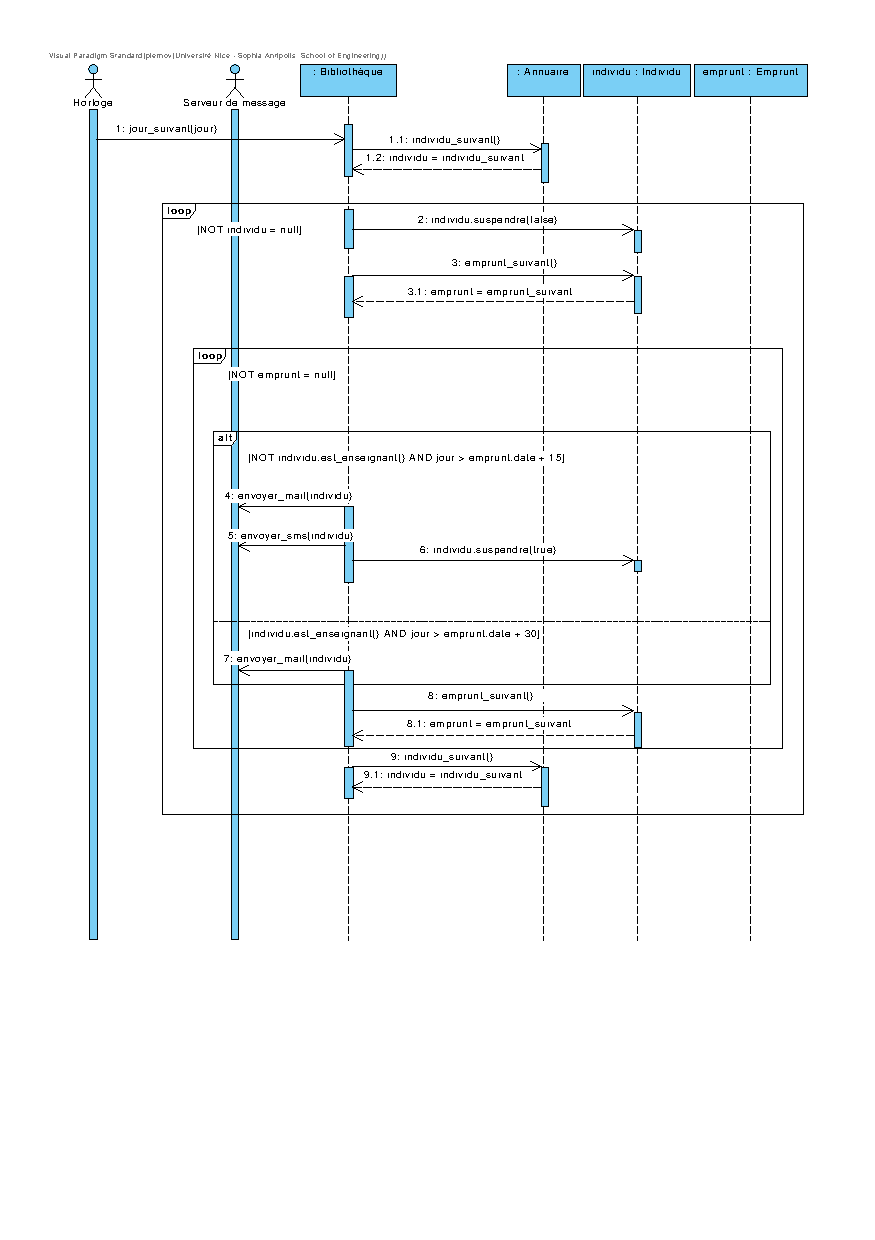
\includegraphics[scale=1.5]{sequence_relancer_pour_rendu_du_livre}
\vspace*{-4em}


\section{Diagrammes d'état}

\section{Auto-évaluation}

\begin{itemize}
	\item \textbf{Cancela Joël}
	\item \textbf{Bounouas Nassim}
	\item \textbf{Mortara Johann}
	\item \textbf{Novac Pierre-Emmanuel}
\end{itemize}

\end{document}
